\documentclass[11pt]{book}

\usepackage{pgf}
\usepackage{tikz}
\usepackage{pgflibraryplotmarks}

\begin{document}
\date{today}


%% Plot generated by GenPlot of alignapi
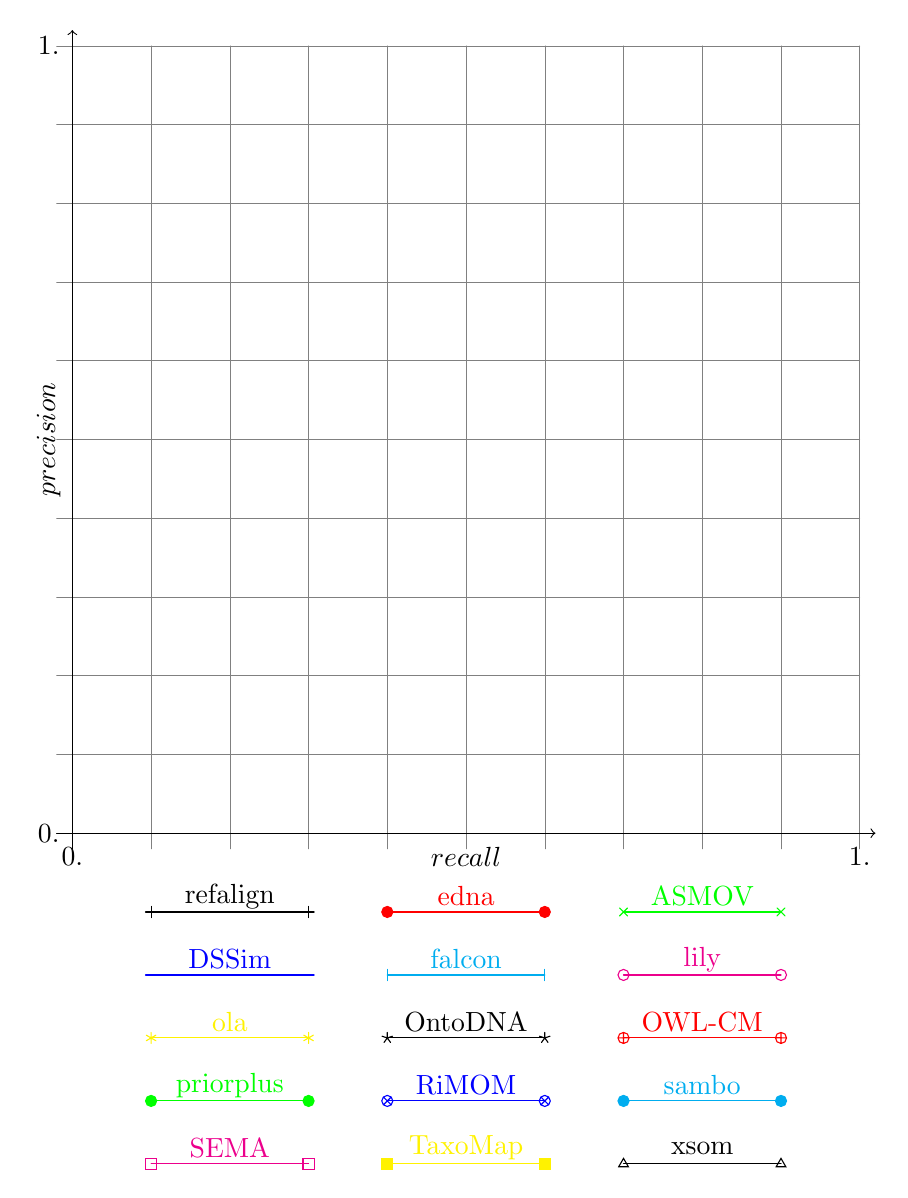
\begin{tikzpicture}[cap=round]
% Draw grid
\draw[step=1cm,very thin,color=gray] (-0.2,-0.2) grid (10,10);
\draw[->] (-0.2,0) -- (10.2,0);
\draw (5,-0.3) node {$recall$}; 
\draw (0,-0.3) node {0.}; 
\draw (10,-0.3) node {1.}; 
\draw[->] (0,-0.2) -- (0,10.2);
\draw (-0.3,0) node {0.}; 
\draw (-0.3,5) node[rotate=90] {$precision$}; 
\draw (-0.3,10) node {1.}; 
% Plots
\draw[black] plot[mark=+,smooth] file {refalign.table};
\draw[red] plot[mark=*,smooth] file {edna.table};
\draw[green] plot[mark=x,smooth] file {ASMOV.table};
\draw[blue] plot[mark=-,smooth] file {DSSim.table};
\draw[cyan] plot[mark=|,smooth] file {falcon.table};
\draw[magenta] plot[mark=o,smooth] file {lily.table};
\draw[yellow] plot[mark=asterisk,smooth] file {ola.table};
\draw[black] plot[mark=star,smooth] file {OntoDNA.table};
\draw[red] plot[mark=oplus,smooth] file {OWL-CM.table};
\draw[green] plot[mark=oplus*,smooth] file {priorplus.table};
\draw[blue] plot[mark=otimes,smooth] file {RiMOM.table};
\draw[cyan] plot[mark=otimes*,smooth] file {sambo.table};
\draw[magenta] plot[mark=square,smooth] file {SEMA.table};
\draw[yellow] plot[mark=square*,smooth] file {TaxoMap.table};
\draw[black] plot[mark=triangle,smooth] file {xsom.table};
% Legend
\draw[black] plot[mark=+,smooth] coordinates {(1,-1.0) (3,-1.0)};
\draw[black] (2,-0.8) node {refalign};
\draw[red] plot[mark=*,smooth] coordinates {(4,-1.0) (6,-1.0)};
\draw[red] (5,-0.8) node {edna};
\draw[green] plot[mark=x,smooth] coordinates {(7,-1.0) (9,-1.0)};
\draw[green] (8,-0.8) node {ASMOV};
\draw[blue] plot[mark=-,smooth] coordinates {(1,-1.8) (3,-1.8)};
\draw[blue] (2,-1.6) node {DSSim};
\draw[cyan] plot[mark=|,smooth] coordinates {(4,-1.8) (6,-1.8)};
\draw[cyan] (5,-1.6) node {falcon};
\draw[magenta] plot[mark=o,smooth] coordinates {(7,-1.8) (9,-1.8)};
\draw[magenta] (8,-1.6) node {lily};
\draw[yellow] plot[mark=asterisk,smooth] coordinates {(1,-2.6) (3,-2.6)};
\draw[yellow] (2,-2.4000000000000004) node {ola};
\draw[black] plot[mark=star,smooth] coordinates {(4,-2.6) (6,-2.6)};
\draw[black] (5,-2.4000000000000004) node {OntoDNA};
\draw[red] plot[mark=oplus,smooth] coordinates {(7,-2.6) (9,-2.6)};
\draw[red] (8,-2.4000000000000004) node {OWL-CM};
\draw[green] plot[mark=oplus*,smooth] coordinates {(1,-3.4000000000000004) (3,-3.4000000000000004)};
\draw[green] (2,-3.2) node {priorplus};
\draw[blue] plot[mark=otimes,smooth] coordinates {(4,-3.4000000000000004) (6,-3.4000000000000004)};
\draw[blue] (5,-3.2) node {RiMOM};
\draw[cyan] plot[mark=otimes*,smooth] coordinates {(7,-3.4000000000000004) (9,-3.4000000000000004)};
\draw[cyan] (8,-3.2) node {sambo};
\draw[magenta] plot[mark=square,smooth] coordinates {(1,-4.2) (3,-4.2)};
\draw[magenta] (2,-4.0) node {SEMA};
\draw[yellow] plot[mark=square*,smooth] coordinates {(4,-4.2) (6,-4.2)};
\draw[yellow] (5,-4.0) node {TaxoMap};
\draw[black] plot[mark=triangle,smooth] coordinates {(7,-4.2) (9,-4.2)};
\draw[black] (8,-4.0) node {xsom};
\end{tikzpicture}

\end{document}
